\documentclass{beamer}
\usepackage[utf8]{inputenc}

\usetheme{Madrid}
\usecolortheme{default}
\usepackage{amsmath,amssymb,amsfonts,amsthm}
\usepackage{mathtools}
\usepackage{txfonts}
\usepackage{tkz-euclide}
\usepackage{listings}
\usepackage{adjustbox}
\usepackage{array}
\usepackage{gensymb}
\usepackage{tabularx}
\usepackage{gvv}
\usepackage{lmodern}
\usepackage{circuitikz}
\usepackage{tikz}
\lstset{literate={·}{{$\cdot$}}1 {λ}{{$\lambda$}}1 {→}{{$\to$}}1}
\usepackage{graphicx}

\setbeamertemplate{page number in head/foot}[totalframenumber]

\usepackage{tcolorbox}
\tcbuselibrary{minted,breakable,xparse,skins}



\definecolor{bg}{gray}{0.95}
\DeclareTCBListing{mintedbox}{O{}m!O{}}{%
  breakable=true,
  listing engine=minted,
  listing only,
  minted language=#2,
  minted style=default,
  minted options={%
    linenos,
    gobble=0,
    breaklines=true,
    breakafter=,,
    fontsize=\small,
    numbersep=8pt,
    #1},
  boxsep=0pt,
  left skip=0pt,
  right skip=0pt,
  left=25pt,
  right=0pt,
  top=3pt,
  bottom=3pt,
  arc=5pt,
  leftrule=0pt,
  rightrule=0pt,
  bottomrule=2pt,
  toprule=2pt,
  colback=bg,
  colframe=orange!70,
  enhanced,
  overlay={%
    \begin{tcbclipinterior}
    \fill[orange!20!white] (frame.south west) rectangle ([xshift=20pt]frame.north west);
    \end{tcbclipinterior}},
  #3,
}
\lstset{
    language=C,
    basicstyle=\ttfamily\small,
    keywordstyle=\color{blue},
    stringstyle=\color{orange},
    commentstyle=\color{green!60!black},
    numbers=left,
    numberstyle=\tiny\color{gray},
    breaklines=true,
    showstringspaces=false,
}
%------------------------------------------------------------
%This block of code defines the information to appear in the
%Title page
\title %optional
{4.13.92}
%\subtitle{A short story}

\author % (optional)
{Pratik R-AI25BTECH11023}



\begin{document}
\frame{\titlepage}
\begin{frame}{Question}
The equation of a plane passing through the line of intersection of the planes $x+2y+3z=2$ and $x-y + z = 3$ and at a distance $\frac{2}{\sqrt{3}}$ from the point $(3,1,-1)$ is 
\end{frame}
\begin{frame}{Solution}
According to the question,\\
\begin{align}
    \vec{n_1}=\myvec{1\\2\\3} \quad \vec{n_2}=\myvec{1\\-1\\1} \quad c_1=2 \quad c_2=3
\end{align}
\end{frame}
\begin{frame}{Solution}
The equation of plane which contains the line of intersection of the two planes is given by
\begin{align}
    \vec{n_1}^{\top}\vec{x}-c_1+\lambda\brak{\vec{n_2}^{\top}\vec{x}-c_2}=0
\end{align}
\begin{align}
    \implies \brak{\vec{n_1}^{\top}+\lambda\vec{n_2}^{\top}}\vec{x}=c_1+\lambda c_2
\end{align}
\end{frame}
\begin{frame}{Solution}
Let $d = \frac{2}{\sqrt{3}}$ be the distance of the plane from the point $P(3,1,-1)$ 
\begin{align}
    \therefore d = \frac{|\brak{\vec{n_1}+\lambda\vec{n_2}}^{\top}\vec{P} - \brak{c_1+\lambda c_2}|}{||\vec{n_1}+\lambda \vec{n_2}||}
\end{align}
simplifying RHS
\begin{align}
    \frac{|2\lambda|}{\sqrt{3\lambda ^2 +4\lambda +14}}
\end{align}
\begin{align}
    \therefore d^2= \frac{4\lambda ^2}{3\lambda ^2 +4\lambda +14}
\end{align}
\end{frame}
\begin{frame}{Solution}
solving this, we get
\begin{align}
   \lambda &=\frac{-7}{2} \text{ or}\\
   \lambda &= \infty
\end{align}
Hence the Equation of plane is given by
\begin{align}
    \myvec{-5&11&-1}\vec{x}=-17
\end{align}
or since $\lambda$ is $\infty$ the plane can be $\vec{n_2}^{\top} \vec{x} = 3 $ itself.
\end{frame}

\begin{frame}{Plot}
    \begin{figure}[H]
    \centering
    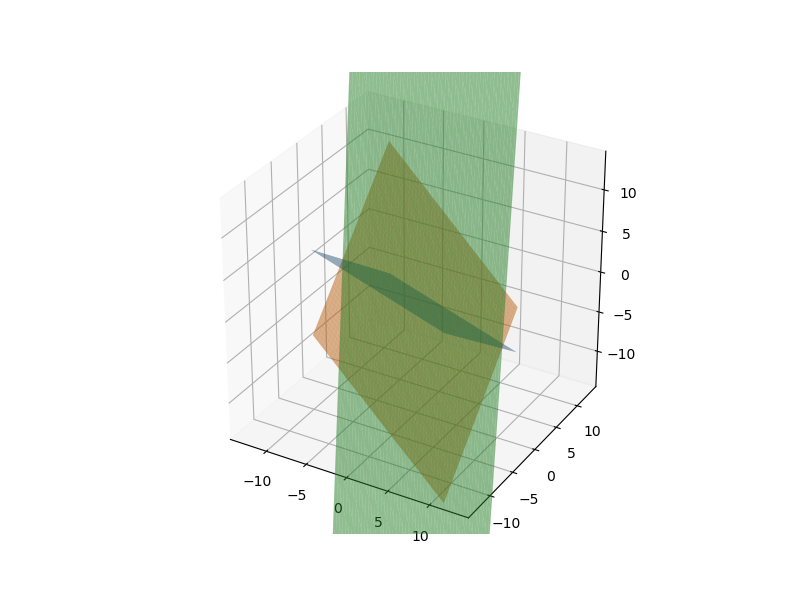
\includegraphics[width=0.6\columnwidth]{../figs/fig.png}
    \label{fig:1}
\end{figure}
\end{frame}

\end{document}